\documentclass[14pt]{beamer}
\author{Daniel Wagner}
\usepackage{tikz}
\usepackage[draft]{beamer_minimal}
\usepackage{presentation}
\usepackage{amssymb}
\usepackage{semantic}
% TODO: related work throughout
% TODO: be clear throughout about collaborators
\begin{document}

% TODO: graphic?
\title{Generalizing Lenses}
\date[University of Pennsylvania]{August 19, 2013}
\maketitle

\begin{frame}
    \frametitle{Thesis Proposal}
    \alert<2>{There are many fundamentally bidirectional settings}
    \alert<3>{that call for generalizations of traditional lenses}
    \alert<4>{where a language is possible and helpful.}
\end{frame}

% TODO: make it clear which bits predate me, which bits I helped with, which
% bits are not yet done
\begin{frame}
    \frametitle{Overview}
    \tableofcontents
\end{frame}

\section{Traditional lenses}
\begin{frame}
    \begin{center}
        \begin{tikzpicture}
            \draw[short picture tree]
                node (root) {} child {
                    node (Jan) {Jan}
                        \lolcatchildren{palindrome,gamer}
                } child {
                    node (May) {May}
                        \lolcatchildren{froghead}
                }
                ;
            \lolcatnotagsdef{froghead-fs-pic}
                {palindrome/{costume,food},gamer/{costume},froghead/{costume}}
            \fswebborder{palindrome}{froghead}
        \end{tikzpicture}
    \end{center}
\end{frame}

\begin{frame}
    \begin{center}
        \begin{tikzpicture}
            \draw[short picture tree]
                node (root) {} child {
                    node (Jan) {Jan}
                        \lolcatchildren{palindrome,gamer}
                } child {
                    node (May) {May}
                        \lolcatchildren{froghead}
                }
                ;
            \lolcatnotagsdef{froghead-fs-pic}
                {palindrome/{costume,food},gamer/{costume},froghead/{costume},burrito/{onlyface}}
            \node[fit=(burrito-web-pic)] (burrito-web-alert) {};
            \path[rounded corners,draw=alertgreen]
                ($(burrito-web-alert.north west) +(0.25,-0.25)$) rectangle
                ($(burrito-web-alert.south east) +(-0.25,0.25)$);
            \fsborder{palindrome}{froghead}
            \webborder{palindrome}{burrito}
        \end{tikzpicture}
    \end{center}
\end{frame}

\begin{frame}
    \begin{center}
        \begin{tikzpicture}
            \draw[short picture tree]
                node (root) {} child {
                    node (Jan) {Jan}
                        \lolcatchildren{palindrome,gamer}
                } child {
                    node (May) {May}
                        \lolcatchildren{froghead}
                } child {
                    node        (burrito-fs-name) {\tiny ???}
                    node[below] (burrito-fs-pic)  {\lolcat{burrito}}
                }
                ;
            \lolcatnotagsdef{burrito-fs-pic}
                {palindrome/{costume,food},gamer/{costume},froghead/{costume},burrito/{onlyface}}
            \fswebborder{palindrome}{burrito}
        \end{tikzpicture}
    \end{center}
\end{frame}

\begin{frame}
    \begin{center}
        \begin{tikzpicture}
            \draw[narrow picture tree]
                node (root) {} child {
                    node (Jan) {Jan}
                        \lolcatchildren{palindrome,gamer}
                } child {
                    node (May) {May}
                        \lolcatchildren{froghead}
                } child[sibling distance=1.33cm] {
                    node        (burrito-fs-name) {\tiny burrito.jpg}
                    node[below] (burrito-fs-pic)  {\lolcat{burrito}}
                } child[sibling distance=1.33cm] {
                    node        (withperson-fs-name) {\tiny withperson.jpg}
                    node[below] (withperson-fs-pic)  {\lolcat{withperson}}
                }
                ;
            \node[fit=(withperson-fs-name) (withperson-fs-pic)] (withperson-fs-alert) {};
            \path[rounded corners,draw=alertgreen]
                ($(withperson-fs-alert.north west) +(0.25,-0.25)$) rectangle
                ($(withperson-fs-alert.south east) +(-0.25,0.25)$);
            \lolcatnotags{(root.north -| withperson-fs-pic.east) +(1.3,0)}
                {palindrome/{costume,food},
                 gamer/{costume},
                 froghead/{costume},
                 burrito/{food,onlyface}}
            \fsborder{palindrome}{withperson}
            \webborder{palindrome}{burrito}
        \end{tikzpicture}
    \end{center}
\end{frame}

\begin{frame}
    \begin{center}
        \begin{tikzpicture}
            \draw[narrow picture tree]
                node (root) {} child {
                    node (Jan) {Jan}
                        \lolcatchildren{palindrome,gamer}
                } child {
                    node (May) {May}
                        \lolcatchildren{froghead}
                } child[sibling distance=1.33cm] {
                    node        (burrito-fs-name) {\tiny burrito.jpg}
                    node[below] (burrito-fs-pic)  {\lolcat{burrito}}
                } child[sibling distance=1.33cm] {
                    node        (withperson-fs-name) {\tiny withperson.jpg}
                    node[below] (withperson-fs-pic)  {\lolcat{withperson}}
                }
                ;
            \lolcatnotags{(root.north -| withperson-fs-pic.east) +(1.3,0)}
                {palindrome/{costume,food},
                 gamer/{costume},
                 froghead/{costume},
                 burrito/{food,onlyface},
                 withperson/{\ }}
             \fswebborder{palindrome}{withperson}
        \end{tikzpicture}
    \end{center}
\end{frame}

\begin{frame}
    % TODO: forgot create!
    \frametitle{Abstract model}
    A lens $\ell \in X \aslens Y$ has components
    \begin{align*}
        get &\in X \to Y \\
        put &\in Y \times X \to X
    \end{align*}
    \pause
    Synchronizing too often doesn't hurt.
    \begin{align*}
        get(put(y,x))&=y \\
        put(get(x),x)&=x \\
        \only<3>{\color{gray}put(y_2,put(y_1,x))&\color{gray}=put(y_2,x)}
    \end{align*}
    \only<3>{\color{gray}Not synchronizing often enough doesn't hurt.}
\end{frame}

% TODO: list the reams of work here on point-free instantiation languages,
% including for strings, relational databases, trees, etc.

\section{Symmetry}
\begin{frame}
    \begin{center}
        \begin{tikzpicture}
            \draw[narrow picture tree]
                node (root) {} child {
                    node (Jan) {Jan}
                        \lolcatchildren{palindrome,gamer}
                } child {
                    node (May) {May}
                        \lolcatchildren{froghead}
                } child[sibling distance=1.33cm] {
                    node        (burrito-fs-name) {\tiny burrito.jpg}
                    node[below] (burrito-fs-pic)  {\lolcat{burrito}}
                } child[sibling distance=1.33cm] {
                    node        (withperson-fs-name) {\tiny withperson.jpg}
                    node[below] (withperson-fs-pic)  {\lolcat{withperson}}
                }
                ;
            \lolcatnotags{(root.north -| withperson-fs-pic.east) +(1.3,0)}
                {palindrome/{costume,food},
                 gamer/{costume},
                 froghead/{costume},
                 burrito/{food,onlyface},
                 withperson/{\ }}
             \fswebborder{palindrome}{withperson}
        \end{tikzpicture}
    \end{center}
\end{frame}

\begin{frame}
    \begin{center}
        \begin{tikzpicture}
            \draw[narrow picture tree]
                node (root) {} child {
                    node (Jan) {Jan}
                        \lolcatchildren{palindrome,gamer}
                } child {
                    node (May) {May}
                        \lolcatchildren{froghead}
                } child[sibling distance=1.33cm] {
                    node        (burrito-fs-name) {\tiny burrito.jpg}
                    node[below] (burrito-fs-pic)  {\lolcat{burrito}}
                } child[sibling distance=1.33cm] {
                    node        (withperson-fs-name) {\tiny withperson.jpg}
                    node[below] (withperson-fs-pic)  {\lolcat{withperson}}
                }
                ;
            \lolcattags{(root.north -| withperson-fs-pic.east) +(1.3,0)}
                {palindrome/{costume,food},
                 gamer/{costume},
                 froghead/{costume},
                 burrito/{food,onlyface},
                 withperson/{\ }}
             \fswebborder{palindrome}{withperson}
        \end{tikzpicture}
    \end{center}
\end{frame}

\begin{frame}
    \begin{center}
        \begin{tikzpicture}
            \draw[narrow picture tree]
                node (root) {} child {
                    node (Jan) {Jan} child {
                        node        (palindrome-fs-name) {\tiny palindrome.jpg}
                        node[below] (palindrome-fs-tag)  {\tiny [costume,food]} (palindrome-fs-tag)
                        node[below] (palindrome-fs-pic)  {\lolcat{palindrome}}
                    } child {
                        node        (gamer-fs-name) {\tiny gamer.jpg}
                        node[below] (gamer-fs-tag)  {\tiny [costume]} (gamer-fs-tag)
                        node[below] (gamer-fs-pic)  {\lolcat{gamer}}
                    }
                } child {
                    node (May) {May} child {
                        node        (froghead-fs-name) {\tiny froghead.jpg}
                        node[below] (froghead-fs-tag)  {\tiny [costume]} (froghead-fs-tag)
                        node[below] (froghead-fs-pic)  {\lolcat{froghead}}
                    }
                } child[sibling distance=1.33cm] {
                    node        (burrito-fs-name) {\tiny burrito.jpg}
                    node[below] (burrito-fs-tag)  {\tiny [food,onlyface]} (burrito-fs-tag)
                    node[below] (burrito-fs-pic)  {\lolcat{burrito}}
                } child[sibling distance=1.33cm] {
                    node        (withperson-fs-name) {\tiny withperson.jpg}
                    node[below] (withperson-fs-tag)  {\tiny [\ ]} (withperson-fs-tag)
                    node[below] (withperson-fs-pic)  {\lolcat{withperson}}
                }
                ;
            \lolcattags{(root.north -| withperson-fs-pic.east) +(1.3,0)}
                {palindrome/{costume,food},
                 gamer/{costume},
                 froghead/{costume},
                 burrito/{food,onlyface},
                 withperson/{\ }}
             \fswebborder{palindrome}{withperson}
             \path[use as bounding box] (fs.north west) -- (web.south east);
             \draw<2>[line width=0.6cm,red!70!black] (fs.center)
                circle (3.2cm)
                +(135:3.2cm) -- +(315:3.2cm)
                ;
        \end{tikzpicture}
    \end{center}
\end{frame}

\begin{frame}
    \begin{center}
        \begin{tikzpicture}
            \draw[narrow picture tree]
                node (root) {} child {
                    node (Jan) {Jan}
                        \lolcatchildren{palindrome,gamer}
                } child {
                    node (May) {May}
                        \lolcatchildren{froghead}
                } child[sibling distance=1.33cm] {
                    node        (burrito-fs-name) {\tiny burrito.jpg}
                    node[below] (burrito-fs-pic)  {\lolcat{burrito}}
                } child[sibling distance=1.33cm] {
                    node        (withperson-fs-name) {\tiny withperson.jpg}
                    node[below] (withperson-fs-pic)  {\lolcat{withperson}}
                }
                ;
            \lolcattags{(root.north -| withperson-fs-pic.east) +(1.3,0)}
                {palindrome/{costume,food},
                 gamer/{costume},
                 froghead/{costume},
                 burrito/{food,onlyface},
                 withperson/{\ }}
             \fswebborder{palindrome}{withperson}
             \path[tiny complement tree] (fs.south) ++(-0.8cm, -0.6cm)
                node (complement-root) {} child {
                    node (complement-Jan) {Jan} child {
                        node (complement-palindrome) {palindrome\strut}
                    } child {
                        node (complement-gamer) {gamer\strut}
                    }
                } child {
                    node (complement-May) {May} child {
                        node (complement-froghead) {froghead\strut}
                    }
                } child {
                    node (complement-burrito) {burrito\strut}
                } child {
                    node (complement-withperson) {withperson\strut}
                }
                ;
                \begin{scope}[start chain=going below,node distance=0,inner sep=0.2ex,font=\tiny]
                    \path (complement-root) ++(3.5cm,-0.1cm)
                        node[on chain] (complement-palindrome-tag) {[costume,food]}
                        node[on chain] (complement-gamer-tag)      {[costume]}
                        node[on chain] (complement-froghead-tag)   {[costume]}
                        node[on chain] (complement-burrito-tag)    {[food,onlyface]}
                        node[on chain] (complement-withperson-tag) {[\ ]}
                        ;
                \end{scope}
                \path<2>
                    node[fit=(complement-root)
                             (complement-palindrome)
                             (complement-palindrome-tag)
                             (complement-withperson-tag)] (complement) {}
                    (complement) node[anchor=center,scale=3] (complement-check)
                        {\Large\color{alertgreen}\checkmark}
                    ;
        \end{tikzpicture}
    \end{center}
\end{frame}

\begin{frame}
    \frametitle{Abstract model}
    A lens $\ell \in X \sslens Y$ has a set $C$ and components
    \begin{align*}
        putr &\in X\times C \to Y\times C \\
        putl &\in Y\times C \to X\times C
    \end{align*}
    \pause
    Synchronizing too often doesn't hurt.
    \[\inference{putr(x,c)=(y,c')}{putl(y,c')=(x,c')}\]
    \pause
    \color{gray}Not synchronizing often enough doesn't hurt.
    \[\inference{putr(x_1,c_0)=(y_1,c_1) \\ putr(x_2,c_1) = (y_2,c_2)}{putr(x_2,c_0)=(y_2,c_2)}\]
\end{frame}

\begin{frame}
    \frametitle{Twist: equational reasoning}
    \begin{center}
        \begin{tikzpicture}[start chain=going right]
            \path
                node[on chain] (A) {A}
                node[on chain] (B) {B}
                node[on chain] (C) {C}
                ;
            \draw[<->] (A) -- node[above] {\tiny$a$} node[below] {$k$}    (B);
            \draw[<->] (B) -- node[above] {\tiny$a$} node[below] {$\ell$} (C);
        \end{tikzpicture}
    \end{center}
    Nice property of asymmetric lenses:
    \[(k;\ell);m = k;(\ell;m)\]
    \pause
    \alert{Not true for symmetric lenses!}
\end{frame}

\begin{frame}
    \frametitle{In dissertation}
    \begin{itemize}
        \item Observational equivalence
        \item Point-free functional programming language
            \begin{itemize}
                \item Basic (non-recursive) data types
                \item Lists, with folds and unfolds
                \item Some generalized container operations
            \end{itemize}
        \item Proof that this generalizes asymmetric lenses
    \end{itemize}
\end{frame}

% TODO: related work

\section{Edits}
\begin{frame}
    \begin{center}
        \begin{tikzpicture}
            \draw[narrow picture tree]
                node (root) {} child {
                    node (Jan) {Jan}
                        \lolcatchildren{palindrome,gamer}
                } child {
                    node (May) {May}
                        \lolcatchildren{froghead}
                } child[sibling distance=1.33cm] {
                    node        (burrito-fs-name) {\tiny burrito.jpg}
                    node[below] (burrito-fs-pic)  {\lolcat{burrito}}
                } child[sibling distance=1.33cm] {
                    node        (withperson-fs-name) {\tiny withperson.jpg}
                    node[below] (withperson-fs-pic)  {\lolcat{withperson}}
                }
                ;
            \lolcattags{(root.north -| withperson-fs-pic.east) +(1.3,0)}
                {palindrome/{costume,food},
                 gamer/{costume},
                 froghead/{costume},
                 burrito/{food,onlyface},
                 withperson/{\ }}
             \fswebborder{palindrome}{withperson}
        \end{tikzpicture}
    \end{center}
\end{frame}

\begin{frame}
    \begin{center}
        \begin{tikzpicture}
% generated by random_cats.hs
\draw[busy picture tree] node (root) {}child{node[inner sep=0,scale=0.5](2012){\strut 2012}child{node[inner sep=0,scale=0.1](January){\strut January}child{node[scale=0.1](first-fs-name){\tiny wrapped.jpg}node[below,scale=0.05](first-fs-pic){\lolcat{wrapped}}}child{node[scale=0.1](last-fs-name){\tiny gamer.jpg}node[below,scale=0.05](last-fs-pic){\lolcat{gamer}}}child{node[scale=0.1](last-fs-name){\tiny froghead.jpg}node[below,scale=0.05](last-fs-pic){\lolcat{froghead}}}}child{node[inner sep=0,scale=0.1](February){\strut February}child{node[scale=0.1](last-fs-name){\tiny wrapped.jpg}node[below,scale=0.05](last-fs-pic){\lolcat{wrapped}}}child{node[scale=0.1](last-fs-name){\tiny burrito.jpg}node[below,scale=0.05](last-fs-pic){\lolcat{burrito}}}child{node[scale=0.1](last-fs-name){\tiny gamer.jpg}node[below,scale=0.05](last-fs-pic){\lolcat{gamer}}}}child{node[inner sep=0,scale=0.1](March){\strut March}child{node[scale=0.1](last-fs-name){\tiny palindrome.jpg}node[below,scale=0.05](last-fs-pic){\lolcat{palindrome}}}child{node[scale=0.1](last-fs-name){\tiny gamer.jpg}node[below,scale=0.05](last-fs-pic){\lolcat{gamer}}}child{node[scale=0.1](last-fs-name){\tiny dune.jpg}node[below,scale=0.05](last-fs-pic){\lolcat{dune}}}child{node[scale=0.1](last-fs-name){\tiny palindrome.jpg}node[below,scale=0.05](last-fs-pic){\lolcat{palindrome}}}child{node[scale=0.1](last-fs-name){\tiny dune.jpg}node[below,scale=0.05](last-fs-pic){\lolcat{dune}}}}child{node[inner sep=0,scale=0.1](April){\strut April}child{node[scale=0.1](last-fs-name){\tiny palindrome.jpg}node[below,scale=0.05](last-fs-pic){\lolcat{palindrome}}}child{node[scale=0.1](last-fs-name){\tiny lobster.jpg}node[below,scale=0.05](last-fs-pic){\lolcat{lobster}}}child{node[scale=0.1](last-fs-name){\tiny withperson.jpg}node[below,scale=0.05](last-fs-pic){\lolcat{withperson}}}}child{node[inner sep=0,scale=0.1](May){\strut May}child{node[scale=0.1](last-fs-name){\tiny wrapped.jpg}node[below,scale=0.05](last-fs-pic){\lolcat{wrapped}}}child{node[scale=0.1](last-fs-name){\tiny dune.jpg}node[below,scale=0.05](last-fs-pic){\lolcat{dune}}}child{node[scale=0.1](last-fs-name){\tiny froghead.jpg}node[below,scale=0.05](last-fs-pic){\lolcat{froghead}}}child{node[scale=0.1](last-fs-name){\tiny dune.jpg}node[below,scale=0.05](last-fs-pic){\lolcat{dune}}}}child{node[inner sep=0,scale=0.1](June){\strut June}child{node[scale=0.1](last-fs-name){\tiny burrito.jpg}node[below,scale=0.05](last-fs-pic){\lolcat{burrito}}}child{node[scale=0.1](last-fs-name){\tiny froghead.jpg}node[below,scale=0.05](last-fs-pic){\lolcat{froghead}}}child{node[scale=0.1](last-fs-name){\tiny gamer.jpg}node[below,scale=0.05](last-fs-pic){\lolcat{gamer}}}child{node[scale=0.1](last-fs-name){\tiny dune.jpg}node[below,scale=0.05](last-fs-pic){\lolcat{dune}}}}child{node[inner sep=0,scale=0.1](July){\strut July}child{node[scale=0.1](last-fs-name){\tiny gamer.jpg}node[below,scale=0.05](last-fs-pic){\lolcat{gamer}}}child{node[scale=0.1](last-fs-name){\tiny froghead.jpg}node[below,scale=0.05](last-fs-pic){\lolcat{froghead}}}child{node[scale=0.1](last-fs-name){\tiny withperson.jpg}node[below,scale=0.05](last-fs-pic){\lolcat{withperson}}}}child{node[inner sep=0,scale=0.1](August){\strut August}child{node[scale=0.1](last-fs-name){\tiny burrito.jpg}node[below,scale=0.05](last-fs-pic){\lolcat{burrito}}}child{node[scale=0.1](last-fs-name){\tiny froghead.jpg}node[below,scale=0.05](last-fs-pic){\lolcat{froghead}}}child{node[scale=0.1](last-fs-name){\tiny dune.jpg}node[below,scale=0.05](last-fs-pic){\lolcat{dune}}}child{node[scale=0.1](last-fs-name){\tiny froghead.jpg}node[below,scale=0.05](last-fs-pic){\lolcat{froghead}}}}child{node[inner sep=0,scale=0.1](September){\strut September}child{node[scale=0.1](last-fs-name){\tiny palindrome.jpg}node[below,scale=0.05](last-fs-pic){\lolcat{palindrome}}}child{node[scale=0.1](last-fs-name){\tiny lobster.jpg}node[below,scale=0.05](last-fs-pic){\lolcat{lobster}}}child{node[scale=0.1](last-fs-name){\tiny gamer.jpg}node[below,scale=0.05](last-fs-pic){\lolcat{gamer}}}}child{node[inner sep=0,scale=0.1](October){\strut October}child{node[scale=0.1](last-fs-name){\tiny withperson.jpg}node[below,scale=0.05](last-fs-pic){\lolcat{withperson}}}child{node[scale=0.1](last-fs-name){\tiny palindrome.jpg}node[below,scale=0.05](last-fs-pic){\lolcat{palindrome}}}child{node[scale=0.1](last-fs-name){\tiny gamer.jpg}node[below,scale=0.05](last-fs-pic){\lolcat{gamer}}}}child{node[inner sep=0,scale=0.1](November){\strut November}child{node[scale=0.1](last-fs-name){\tiny froghead.jpg}node[below,scale=0.05](last-fs-pic){\lolcat{froghead}}}child{node[scale=0.1](last-fs-name){\tiny burrito.jpg}node[below,scale=0.05](last-fs-pic){\lolcat{burrito}}}child{node[scale=0.1](last-fs-name){\tiny gamer.jpg}node[below,scale=0.05](last-fs-pic){\lolcat{gamer}}}child{node[scale=0.1](last-fs-name){\tiny burrito.jpg}node[below,scale=0.05](last-fs-pic){\lolcat{burrito}}}child{node[scale=0.1](last-fs-name){\tiny withperson.jpg}node[below,scale=0.05](last-fs-pic){\lolcat{withperson}}}}child{node[inner sep=0,scale=0.1](December){\strut December}child{node[scale=0.1](last-fs-name){\tiny gamer.jpg}node[below,scale=0.05](last-fs-pic){\lolcat{gamer}}}child{node[scale=0.1](last-fs-name){\tiny wrapped.jpg}node[below,scale=0.05](last-fs-pic){\lolcat{wrapped}}}child{node[scale=0.1](last-fs-name){\tiny dune.jpg}node[below,scale=0.05](last-fs-pic){\lolcat{dune}}}child{node[scale=0.1](last-fs-name){\tiny lobster.jpg}node[below,scale=0.05](last-fs-pic){\lolcat{lobster}}}}}child{node[inner sep=0,scale=0.5](2013){\strut 2013}child{node[inner sep=0,scale=0.1](January){\strut January}child{node[scale=0.1](last-fs-name){\tiny froghead.jpg}node[below,scale=0.05](last-fs-pic){\lolcat{froghead}}}child{node[scale=0.1](last-fs-name){\tiny withperson.jpg}node[below,scale=0.05](last-fs-pic){\lolcat{withperson}}}child{node[scale=0.1](last-fs-name){\tiny palindrome.jpg}node[below,scale=0.05](last-fs-pic){\lolcat{palindrome}}}child{node[scale=0.1](last-fs-name){\tiny wrapped.jpg}node[below,scale=0.05](last-fs-pic){\lolcat{wrapped}}}}child{node[inner sep=0,scale=0.1](February){\strut February}child{node[scale=0.1](last-fs-name){\tiny dune.jpg}node[below,scale=0.05](last-fs-pic){\lolcat{dune}}}child{node[scale=0.1](last-fs-name){\tiny froghead.jpg}node[below,scale=0.05](last-fs-pic){\lolcat{froghead}}}child{node[scale=0.1](last-fs-name){\tiny palindrome.jpg}node[below,scale=0.05](last-fs-pic){\lolcat{palindrome}}}}child{node[inner sep=0,scale=0.1](March){\strut March}child{node[scale=0.1](last-fs-name){\tiny lobster.jpg}node[below,scale=0.05](last-fs-pic){\lolcat{lobster}}}child{node[scale=0.1](last-fs-name){\tiny froghead.jpg}node[below,scale=0.05](last-fs-pic){\lolcat{froghead}}}child{node[scale=0.1](last-fs-name){\tiny palindrome.jpg}node[below,scale=0.05](last-fs-pic){\lolcat{palindrome}}}}child{node[inner sep=0,scale=0.1](April){\strut April}child{node[scale=0.1](last-fs-name){\tiny dune.jpg}node[below,scale=0.05](last-fs-pic){\lolcat{dune}}}child{node[scale=0.1](last-fs-name){\tiny gamer.jpg}node[below,scale=0.05](last-fs-pic){\lolcat{gamer}}}child{node[scale=0.1](last-fs-name){\tiny withperson.jpg}node[below,scale=0.05](last-fs-pic){\lolcat{withperson}}}child{node[scale=0.1](last-fs-name){\tiny dune.jpg}node[below,scale=0.05](last-fs-pic){\lolcat{dune}}}child{node[scale=0.1](last-fs-name){\tiny wrapped.jpg}node[below,scale=0.05](last-fs-pic){\lolcat{wrapped}}}}child{node[inner sep=0,scale=0.1](May){\strut May}child{node[scale=0.1](last-fs-name){\tiny withperson.jpg}node[below,scale=0.05](last-fs-pic){\lolcat{withperson}}}child{node[scale=0.1](last-fs-name){\tiny burrito.jpg}node[below,scale=0.05](last-fs-pic){\lolcat{burrito}}}child{node[scale=0.1](last-fs-name){\tiny withperson.jpg}node[below,scale=0.05](last-fs-pic){\lolcat{withperson}}}child{node[scale=0.1](last-fs-name){\tiny froghead.jpg}node[below,scale=0.05](last-fs-pic){\lolcat{froghead}}}child{node[scale=0.1](last-fs-name){\tiny lobster.jpg}node[below,scale=0.05](last-fs-pic){\lolcat{lobster}}}}child{node[inner sep=0,scale=0.1](June){\strut June}child{node[scale=0.1](last-fs-name){\tiny wrapped.jpg}node[below,scale=0.05](last-fs-pic){\lolcat{wrapped}}}child{node[scale=0.1](last-fs-name){\tiny burrito.jpg}node[below,scale=0.05](last-fs-pic){\lolcat{burrito}}}child{node[scale=0.1](last-fs-name){\tiny wrapped.jpg}node[below,scale=0.05](last-fs-pic){\lolcat{wrapped}}}child{node[scale=0.1](last-fs-name){\tiny palindrome.jpg}node[below,scale=0.05](last-fs-pic){\lolcat{palindrome}}}child{node[scale=0.1](last-fs-name){\tiny burrito.jpg}node[below,scale=0.05](last-fs-pic){\lolcat{burrito}}}}child{node[inner sep=0,scale=0.1](July){\strut July}child{node[scale=0.1](last-fs-name){\tiny palindrome.jpg}node[below,scale=0.05](last-fs-pic){\lolcat{palindrome}}}child{node[scale=0.1](last-fs-name){\tiny withperson.jpg}node[below,scale=0.05](last-fs-pic){\lolcat{withperson}}}child{node[scale=0.1](last-fs-name){\tiny burrito.jpg}node[below,scale=0.05](last-fs-pic){\lolcat{burrito}}}child{node[scale=0.1](last-fs-name){\tiny wrapped.jpg}node[below,scale=0.05](last-fs-pic){\lolcat{wrapped}}}}child{node[inner sep=0,scale=0.1](August){\strut August}child{node[scale=0.1](last-fs-name){\tiny gamer.jpg}node[below,scale=0.05](last-fs-pic){\lolcat{gamer}}}child{node[scale=0.1](last-fs-name){\tiny froghead.jpg}node[below,scale=0.05](last-fs-pic){\lolcat{froghead}}}child{node[scale=0.1](last-fs-name){\tiny wrapped.jpg}node[below,scale=0.05](last-fs-pic){\lolcat{wrapped}}}child{node[scale=0.1](last-fs-name){\tiny withperson.jpg}node[below,scale=0.05](last-fs-pic){\lolcat{withperson}}}child{node[scale=0.1](last-fs-name){\tiny gamer.jpg}node[below,scale=0.05](last-fs-pic){\lolcat{gamer}}}}child{node[inner sep=0,scale=0.1](September){\strut September}child{node[scale=0.1](last-fs-name){\tiny froghead.jpg}node[below,scale=0.05](last-fs-pic){\lolcat{froghead}}}child{node[scale=0.1](last-fs-name){\tiny lobster.jpg}node[below,scale=0.05](last-fs-pic){\lolcat{lobster}}}child{node[scale=0.1](last-fs-name){\tiny palindrome.jpg}node[below,scale=0.05](last-fs-pic){\lolcat{palindrome}}}child{node[scale=0.1](last-fs-name){\tiny gamer.jpg}node[below,scale=0.05](last-fs-pic){\lolcat{gamer}}}child{node[scale=0.1](last-fs-name){\tiny burrito.jpg}node[below,scale=0.05](last-fs-pic){\lolcat{burrito}}}}child{node[inner sep=0,scale=0.1](October){\strut October}child{node[scale=0.1](last-fs-name){\tiny froghead.jpg}node[below,scale=0.05](last-fs-pic){\lolcat{froghead}}}child{node[scale=0.1](last-fs-name){\tiny withperson.jpg}node[below,scale=0.05](last-fs-pic){\lolcat{withperson}}}child{node[scale=0.1](last-fs-name){\tiny dune.jpg}node[below,scale=0.05](last-fs-pic){\lolcat{dune}}}}child{node[inner sep=0,scale=0.1](November){\strut November}child{node[scale=0.1](last-fs-name){\tiny burrito.jpg}node[below,scale=0.05](last-fs-pic){\lolcat{burrito}}}child{node[scale=0.1](last-fs-name){\tiny withperson.jpg}node[below,scale=0.05](last-fs-pic){\lolcat{withperson}}}child{node[scale=0.1](last-fs-name){\tiny wrapped.jpg}node[below,scale=0.05](last-fs-pic){\lolcat{wrapped}}}}child{node[inner sep=0,scale=0.1](December){\strut December}child{node[scale=0.1](last-fs-name){\tiny froghead.jpg}node[below,scale=0.05](last-fs-pic){\lolcat{froghead}}}child{node[scale=0.1](last-fs-name){\tiny burrito.jpg}node[below,scale=0.05](last-fs-pic){\lolcat{burrito}}}child{node[scale=0.1](last-fs-name){\tiny froghead.jpg}node[below,scale=0.05](last-fs-pic){\lolcat{froghead}}}}};\fsborder{first}{last}\begin{scope}[start chain=going below,node distance=0]\draw(root.north -| last-fs-pic.east) +(1.3,0)node[on chain,anchor=north,scale=0.06](first-web-pic){\lolcat{wrapped}}node[right=of first-web-pic,scale=0.06](first-web-tag){\tiny [cute]}node[on chain,anchor=north,scale=0.06](last-web-pic){\lolcat{gamer}}node[right=of last-web-pic,scale=0.06](last-web-tag){\tiny [kitten,invisible,apathy]}node[on chain,anchor=north,scale=0.06](last-web-pic){\lolcat{froghead}}node[right=of last-web-pic,scale=0.06](last-web-tag){\tiny [food,costume,cute]}node[on chain,anchor=north,scale=0.06](last-web-pic){\lolcat{wrapped}}node[right=of last-web-pic,scale=0.06](last-web-tag){\tiny [food]}node[on chain,anchor=north,scale=0.06](last-web-pic){\lolcat{burrito}}node[right=of last-web-pic,scale=0.06](last-web-tag){\tiny [costume]}node[on chain,anchor=north,scale=0.06](last-web-pic){\lolcat{gamer}}node[right=of last-web-pic,scale=0.06](last-web-tag){\tiny [dog,kitten]}node[on chain,anchor=north,scale=0.06](last-web-pic){\lolcat{palindrome}}node[right=of last-web-pic,scale=0.06](last-web-tag){\tiny [food]}node[on chain,anchor=north,scale=0.06](last-web-pic){\lolcat{gamer}}node[right=of last-web-pic,scale=0.06](last-web-tag){\tiny [invisible,food]}node[on chain,anchor=north,scale=0.06](last-web-pic){\lolcat{dune}}node[right=of last-web-pic,scale=0.06](last-web-tag){\tiny [food,cute]}node[on chain,anchor=north,scale=0.06](last-web-pic){\lolcat{palindrome}}node[right=of last-web-pic,scale=0.06](last-web-tag){\tiny [food,cute]}node[on chain,anchor=north,scale=0.06](last-web-pic){\lolcat{dune}}node[right=of last-web-pic,scale=0.06](last-web-tag){\tiny [\ ]}node[on chain,anchor=north,scale=0.06](last-web-pic){\lolcat{palindrome}}node[right=of last-web-pic,scale=0.06](last-web-tag){\tiny [\ ]}node[on chain,anchor=north,scale=0.06](last-web-pic){\lolcat{lobster}}node[right=of last-web-pic,scale=0.06](last-web-tag){\tiny [costume,dog]}node[on chain,anchor=north,scale=0.06](last-web-pic){\lolcat{withperson}}node[right=of last-web-pic,scale=0.06](last-web-tag){\tiny [dog,kitten,invisible]}node[on chain,anchor=north,scale=0.06](last-web-pic){\lolcat{wrapped}}node[right=of last-web-pic,scale=0.06](last-web-tag){\tiny [\ ]}node[on chain,anchor=north,scale=0.06](last-web-pic){\lolcat{dune}}node[right=of last-web-pic,scale=0.06](last-web-tag){\tiny [\ ]}node[on chain,anchor=north,scale=0.06](last-web-pic){\lolcat{froghead}}node[right=of last-web-pic,scale=0.06](last-web-tag){\tiny [\ ]}node[on chain,anchor=north,scale=0.06](last-web-pic){\lolcat{dune}}node[right=of last-web-pic,scale=0.06](last-web-tag){\tiny [\ ]}node[on chain,anchor=north,scale=0.06](last-web-pic){\lolcat{burrito}}node[right=of last-web-pic,scale=0.06](last-web-tag){\tiny [\ ]}node[on chain,anchor=north,scale=0.06](last-web-pic){\lolcat{froghead}}node[right=of last-web-pic,scale=0.06](last-web-tag){\tiny [food,dog]}node[on chain,anchor=north,scale=0.06](last-web-pic){\lolcat{gamer}}node[right=of last-web-pic,scale=0.06](last-web-tag){\tiny [\ ]}node[on chain,anchor=north,scale=0.06](last-web-pic){\lolcat{dune}}node[right=of last-web-pic,scale=0.06](last-web-tag){\tiny [kitten]}node[on chain,anchor=north,scale=0.06](last-web-pic){\lolcat{gamer}}node[right=of last-web-pic,scale=0.06](last-web-tag){\tiny [\ ]}node[on chain,anchor=north,scale=0.06](last-web-pic){\lolcat{froghead}}node[right=of last-web-pic,scale=0.06](last-web-tag){\tiny [\ ]}node[on chain,anchor=north,scale=0.06](last-web-pic){\lolcat{withperson}}node[right=of last-web-pic,scale=0.06](last-web-tag){\tiny [invisible,cute,costume]}node[on chain,anchor=north,scale=0.06](last-web-pic){\lolcat{burrito}}node[right=of last-web-pic,scale=0.06](last-web-tag){\tiny [\ ]}node[on chain,anchor=north,scale=0.06](last-web-pic){\lolcat{froghead}}node[right=of last-web-pic,scale=0.06](last-web-tag){\tiny [\ ]}node[on chain,anchor=north,scale=0.06](last-web-pic){\lolcat{dune}}node[right=of last-web-pic,scale=0.06](last-web-tag){\tiny [food,invisible]}node[on chain,anchor=north,scale=0.06](last-web-pic){\lolcat{froghead}}node[right=of last-web-pic,scale=0.06](last-web-tag){\tiny [kitten,dog]}node[on chain,anchor=north,scale=0.06](last-web-pic){\lolcat{palindrome}}node[right=of last-web-pic,scale=0.06](last-web-tag){\tiny [invisible,kitten]}node[on chain,anchor=north,scale=0.06](last-web-pic){\lolcat{lobster}}node[right=of last-web-pic,scale=0.06](last-web-tag){\tiny [costume,cute,onlyface]}node[on chain,anchor=north,scale=0.06](last-web-pic){\lolcat{gamer}}node[right=of last-web-pic,scale=0.06](last-web-tag){\tiny [cute]}node[on chain,anchor=north,scale=0.06](last-web-pic){\lolcat{withperson}}node[right=of last-web-pic,scale=0.06](last-web-tag){\tiny [\ ]}node[on chain,anchor=north,scale=0.06](last-web-pic){\lolcat{palindrome}}node[right=of last-web-pic,scale=0.06](last-web-tag){\tiny [\ ]}node[on chain,anchor=north,scale=0.06](last-web-pic){\lolcat{gamer}}node[right=of last-web-pic,scale=0.06](last-web-tag){\tiny [onlyface]}node[on chain,anchor=north,scale=0.06](last-web-pic){\lolcat{froghead}}node[right=of last-web-pic,scale=0.06](last-web-tag){\tiny [invisible,onlyface]}node[on chain,anchor=north,scale=0.06](last-web-pic){\lolcat{burrito}}node[right=of last-web-pic,scale=0.06](last-web-tag){\tiny [\ ]}node[on chain,anchor=north,scale=0.06](last-web-pic){\lolcat{gamer}}node[right=of last-web-pic,scale=0.06](last-web-tag){\tiny [\ ]}node[on chain,anchor=north,scale=0.06](last-web-pic){\lolcat{burrito}}node[right=of last-web-pic,scale=0.06](last-web-tag){\tiny [cute]}node[on chain,anchor=north,scale=0.06](last-web-pic){\lolcat{withperson}}node[right=of last-web-pic,scale=0.06](last-web-tag){\tiny [\ ]}node[on chain,anchor=north,scale=0.06](last-web-pic){\lolcat{gamer}}node[right=of last-web-pic,scale=0.06](last-web-tag){\tiny [dog,cute]}node[on chain,anchor=north,scale=0.06](last-web-pic){\lolcat{wrapped}}node[right=of last-web-pic,scale=0.06](last-web-tag){\tiny [\ ]}node[on chain,anchor=north,scale=0.06](last-web-pic){\lolcat{dune}}node[right=of last-web-pic,scale=0.06](last-web-tag){\tiny [costume]}node[on chain,anchor=north,scale=0.06](last-web-pic){\lolcat{lobster}}node[right=of last-web-pic,scale=0.06](last-web-tag){\tiny [\ ]}node[on chain,anchor=north,scale=0.06](last-web-pic){\lolcat{froghead}}node[right=of last-web-pic,scale=0.06](last-web-tag){\tiny [\ ]}node[on chain,anchor=north,scale=0.06](last-web-pic){\lolcat{withperson}}node[right=of last-web-pic,scale=0.06](last-web-tag){\tiny [\ ]}node[on chain,anchor=north,scale=0.06](last-web-pic){\lolcat{palindrome}}node[right=of last-web-pic,scale=0.06](last-web-tag){\tiny [kitten,apathy,cute]}node[on chain,anchor=north,scale=0.06](last-web-pic){\lolcat{wrapped}}node[right=of last-web-pic,scale=0.06](last-web-tag){\tiny [\ ]}node[on chain,anchor=north,scale=0.06](last-web-pic){\lolcat{dune}}node[right=of last-web-pic,scale=0.06](last-web-tag){\tiny [onlyface]}node[on chain,anchor=north,scale=0.06](last-web-pic){\lolcat{froghead}}node[right=of last-web-pic,scale=0.06](last-web-tag){\tiny [\ ]}node[on chain,anchor=north,scale=0.06](last-web-pic){\lolcat{palindrome}}node[right=of last-web-pic,scale=0.06](last-web-tag){\tiny [food,cute,invisible]}node[on chain,anchor=north,scale=0.06](last-web-pic){\lolcat{lobster}}node[right=of last-web-pic,scale=0.06](last-web-tag){\tiny [invisible,apathy,costume]}node[on chain,anchor=north,scale=0.06](last-web-pic){\lolcat{froghead}}node[right=of last-web-pic,scale=0.06](last-web-tag){\tiny [dog]}node[on chain,anchor=north,scale=0.06](last-web-pic){\lolcat{palindrome}}node[right=of last-web-pic,scale=0.06](last-web-tag){\tiny [costume,dog]}node[on chain,anchor=north,scale=0.06](last-web-pic){\lolcat{dune}}node[right=of last-web-pic,scale=0.06](last-web-tag){\tiny [\ ]}node[on chain,anchor=north,scale=0.06](last-web-pic){\lolcat{gamer}}node[right=of last-web-pic,scale=0.06](last-web-tag){\tiny [dog]}node[on chain,anchor=north,scale=0.06](last-web-pic){\lolcat{withperson}}node[right=of last-web-pic,scale=0.06](last-web-tag){\tiny [apathy]}node[on chain,anchor=north,scale=0.06](last-web-pic){\lolcat{dune}}node[right=of last-web-pic,scale=0.06](last-web-tag){\tiny [onlyface]}node[on chain,anchor=north,scale=0.06](last-web-pic){\lolcat{wrapped}}node[right=of last-web-pic,scale=0.06](last-web-tag){\tiny [kitten]}node[on chain,anchor=north,scale=0.06](last-web-pic){\lolcat{withperson}}node[right=of last-web-pic,scale=0.06](last-web-tag){\tiny [costume,apathy]}node[on chain,anchor=north,scale=0.06](last-web-pic){\lolcat{burrito}}node[right=of last-web-pic,scale=0.06](last-web-tag){\tiny [invisible,onlyface]}node[on chain,anchor=north,scale=0.06](last-web-pic){\lolcat{withperson}}node[right=of last-web-pic,scale=0.06](last-web-tag){\tiny [kitten,onlyface,apathy]}node[on chain,anchor=north,scale=0.06](last-web-pic){\lolcat{froghead}}node[right=of last-web-pic,scale=0.06](last-web-tag){\tiny [apathy,cute,onlyface]}node[on chain,anchor=north,scale=0.06](last-web-pic){\lolcat{lobster}}node[right=of last-web-pic,scale=0.06](last-web-tag){\tiny [costume,apathy]}node[on chain,anchor=north,scale=0.06](last-web-pic){\lolcat{wrapped}}node[right=of last-web-pic,scale=0.06](last-web-tag){\tiny [onlyface,cute,invisible]}node[on chain,anchor=north,scale=0.06](last-web-pic){\lolcat{burrito}}node[right=of last-web-pic,scale=0.06](last-web-tag){\tiny [costume]}node[on chain,anchor=north,scale=0.06](last-web-pic){\lolcat{wrapped}}node[right=of last-web-pic,scale=0.06](last-web-tag){\tiny [apathy,onlyface,costume]}node[on chain,anchor=north,scale=0.06](last-web-pic){\lolcat{palindrome}}node[right=of last-web-pic,scale=0.06](last-web-tag){\tiny [cute]}node[on chain,anchor=north,scale=0.06](last-web-pic){\lolcat{burrito}}node[right=of last-web-pic,scale=0.06](last-web-tag){\tiny [cute,kitten]}node[on chain,anchor=north,scale=0.06](last-web-pic){\lolcat{palindrome}}node[right=of last-web-pic,scale=0.06](last-web-tag){\tiny [\ ]}node[on chain,anchor=north,scale=0.06](last-web-pic){\lolcat{withperson}}node[right=of last-web-pic,scale=0.06](last-web-tag){\tiny [\ ]}node[on chain,anchor=north,scale=0.06](last-web-pic){\lolcat{burrito}}node[right=of last-web-pic,scale=0.06](last-web-tag){\tiny [costume]}node[on chain,anchor=north,scale=0.06](last-web-pic){\lolcat{wrapped}}node[right=of last-web-pic,scale=0.06](last-web-tag){\tiny [\ ]}node[on chain,anchor=north,scale=0.06](last-web-pic){\lolcat{gamer}}node[right=of last-web-pic,scale=0.06](last-web-tag){\tiny [invisible]}node[on chain,anchor=north,scale=0.06](last-web-pic){\lolcat{froghead}}node[right=of last-web-pic,scale=0.06](last-web-tag){\tiny [invisible]}node[on chain,anchor=north,scale=0.06](last-web-pic){\lolcat{wrapped}}node[right=of last-web-pic,scale=0.06](last-web-tag){\tiny [apathy,dog]}node[on chain,anchor=north,scale=0.06](last-web-pic){\lolcat{withperson}}node[right=of last-web-pic,scale=0.06](last-web-tag){\tiny [onlyface]}node[on chain,anchor=north,scale=0.06](last-web-pic){\lolcat{gamer}}node[right=of last-web-pic,scale=0.06](last-web-tag){\tiny [\ ]}node[on chain,anchor=north,scale=0.06](last-web-pic){\lolcat{froghead}}node[right=of last-web-pic,scale=0.06](last-web-tag){\tiny [costume,kitten]}node[on chain,anchor=north,scale=0.06](last-web-pic){\lolcat{lobster}}node[right=of last-web-pic,scale=0.06](last-web-tag){\tiny [food,onlyface]}node[on chain,anchor=north,scale=0.06](last-web-pic){\lolcat{palindrome}}node[right=of last-web-pic,scale=0.06](last-web-tag){\tiny [apathy]}node[on chain,anchor=north,scale=0.06](last-web-pic){\lolcat{gamer}}node[right=of last-web-pic,scale=0.06](last-web-tag){\tiny [onlyface,food]}node[on chain,anchor=north,scale=0.06](last-web-pic){\lolcat{burrito}}node[right=of last-web-pic,scale=0.06](last-web-tag){\tiny [invisible,apathy,costume]}node[on chain,anchor=north,scale=0.06](last-web-pic){\lolcat{froghead}}node[right=of last-web-pic,scale=0.06](last-web-tag){\tiny [onlyface,kitten]}node[on chain,anchor=north,scale=0.06](last-web-pic){\lolcat{withperson}}node[right=of last-web-pic,scale=0.06](last-web-tag){\tiny [\ ]}node[on chain,anchor=north,scale=0.06](last-web-pic){\lolcat{dune}}node[right=of last-web-pic,scale=0.06](last-web-tag){\tiny [\ ]}node[on chain,anchor=north,scale=0.06](last-web-pic){\lolcat{burrito}}node[right=of last-web-pic,scale=0.06](last-web-tag){\tiny [food,onlyface]}node[on chain,anchor=north,scale=0.06](last-web-pic){\lolcat{withperson}}node[right=of last-web-pic,scale=0.06](last-web-tag){\tiny [cute,apathy]}node[on chain,anchor=north,scale=0.06](last-web-pic){\lolcat{wrapped}}node[right=of last-web-pic,scale=0.06](last-web-tag){\tiny [\ ]}node[on chain,anchor=north,scale=0.06](last-web-pic){\lolcat{froghead}}node[right=of last-web-pic,scale=0.06](last-web-tag){\tiny [dog,costume]}node[on chain,anchor=north,scale=0.06](last-web-pic){\lolcat{burrito}}node[right=of last-web-pic,scale=0.06](last-web-tag){\tiny [cute,food]}node[on chain,anchor=north,scale=0.06](last-web-pic){\lolcat{froghead}}node[right=of last-web-pic,scale=0.06](last-web-tag){\tiny [kitten,costume]};\end{scope}\webborder{first}{last}
        \end{tikzpicture}
    \end{center}
\end{frame}

\begin{frame}
    \frametitle{Abstract model}
    Edit lens $\ell \in (M,X,\cdot) \selens (N,Y,\odot)$ has set $C$ and
    \begin{align*}
        dputr &\in M \times C \to N \times C \\
        dputl &\in N \times C \to M \times C
    \end{align*}
    \pause
    Synchronizing too often doesn't hurt.
    \[dputr(\ONE_M,c) = (\ONE_N,c)\]
    \pause
    Not synchronizing often enough doesn't hurt.
    \[\inference{dputr(m,c)=(n,c') \\ dputr(m',c')=(n',c'')}{dputr(mm',c)=(nn',c'')}\]
\end{frame}

\begin{frame}
    \frametitle{Notable benefits}
    \begin{itemize}
        \item All changes reported, so synchronizing less often is less controversial
        \item Intentional information in edits aids alignment
        \item Smaller complement in many cases!
        \item Roundtrip laws are monoid homomorphism laws
            \pause
        \item Observational equivalence, combinator language, generalizes
            symmetric lenses
    \end{itemize}
\end{frame}

% TODO: related work

\section{Multidirectionality}
% TODO: deduplicate using beamer's method of setting up pointers and whatnot
\begin{frame}
    \begin{center}
        \begin{tikzpicture}
            \draw[narrow picture tree]
                node (root) {} child {
                    node (Jan) {Jan}
                        \lolcatchildren{palindrome,gamer}
                } child {
                    node (May) {May}
                        \lolcatchildren{froghead}
                } child[sibling distance=1.33cm] {
                    node        (burrito-fs-name) {\tiny burrito.jpg}
                    node[below] (burrito-fs-pic)  {\lolcat{burrito}}
                } child[sibling distance=1.33cm] {
                    node        (withperson-fs-name) {\tiny withperson.jpg}
                    node[below] (withperson-fs-pic)  {\lolcat{withperson}}
                }
                ;
            \lolcattags{(root.north -| withperson-fs-pic.east) +(1.3,0)}
                {palindrome/{costume,food},
                 gamer/{costume},
                 froghead/{costume},
                 burrito/{food,onlyface},
                 withperson/{\ }}
             \fswebborder{palindrome}{withperson}
        \end{tikzpicture}
    \end{center}
\end{frame}

\begin{frame}
    \begin{center}
        \begin{tikzpicture}
            \lolcattags{}
                {palindrome/{costume,food},
                 gamer/{costume},
                 froghead/{costume},
                 burrito/{food,onlyface},
                 withperson/{\ }}
            \webborder{palindrome}{withperson}
            \lolcatnotags{(palindrome-web-pic.north east) ++(4,0)}
                {palindrome/{},
                 gamer/{},
                 froghead/{}}
            \webborder{palindrome}{froghead}
            \path (web.south) node[below] {costume};
            \lolcatnotags{(palindrome-web-pic.north east) ++(2,0)}
                {palindrome/{},
                 burrito/{}}
            \webborder{palindrome}{burrito}
            \path (web.south) node[below] {food};
            \lolcatnotags{(burrito-web-pic.south) ++(0,-1.5)}
                {burrito/{}}
            \webborder{burrito}{burrito}
            \path (web.south) node[below] {onlyface};
        \end{tikzpicture}
    \end{center}
\end{frame}

\begin{frame}
    \begin{center}
        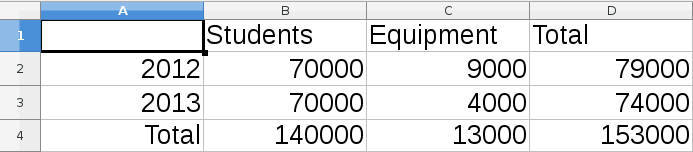
\includegraphics[scale=0.5]{images/spreadsheet.png}
    \end{center}
\end{frame}

\section{Logistics}
\end{document}
